\chapter{Esperimenti}

\section{Cluster ChemGrid}

Tutti gli esperimenti sono stati eseguiti sul cluster ChemGrid. Il cluster \`{e} composto da 11 nodi a 32 bit con 2 processori Intel(R) Pentium(R) 4 CPU 3.06GHz. Tutti i nodi hanno 1GB di memoria tranne 4 nodi (8, 9 10, 11) che hanno 4GB. 3 nodi (3, 6, 11) sono offline e dunque non utilizzabili per sottomettere job. Dunque i nodi utilizzabili sono 8 per un totale di 16 CPU.

Da ricordare che ci serve un quadrato perfetto per eseguire l'algoritmo di Cannon: 4, 9 e 16 sono i possibili candidati. 9 non \`{e} possibile utilizzarlo perch \`{e} non si hanno a disposizione sufficienti host.
Il 4 potrebbe essere derivato da 4 host con una sola CPU oppure da 2 host con 2 CPU. Infine 16 \`{e} ottenibile solo con 8 host a 2 CPU l'uno.
Tutti gli esperimenti verranno eseguiti con questa ultima configurazione: 8 host e 2 CPU per nodo, per un totale di 16 CPU.

\section{Data file}

Il file di input utilizzato per gli esperimenti ha le seguenti dimensioni:

\begin{lstlisting}
4 4 4 2
8 8 8 2
16 16 16 2
32 32 32 2
64 64 64 2
128 128 128 2
192 192 192 2
256 256 256 2
384 384 384 2
512 512 512 2
768 768 768 2
1024 1024 1024 2
1536 1536 1536 2
2048 2048 2048 2
3072 3072 3072 2
4096 4096 4096 2
\end{lstlisting}

Non ha senso andare oltre 4096 perch\`{e} la computazione inizia ad essere impegnativa impiegando tutte le risorse del cluster. Si consideri che una matrice quadrata con n = 4096 ha 134217728 elementi. Ogni elemento \`{e} un double che occupa 8 bytes, dunque una matrice occupa circa 131Mb.
Tutti i test sono stati fatti utilizzando 2 iterazioni.

\subsection{Seriale}

La versione seriale \`{e} stata eseguita su un nodo (cg11) che ha 4GB di memoria per permettere alle dimensioni pi\`{u} grandi si essere moltiplicate senza problemi. Di seguito i dati dei suoi risultati:

\begin{lstlisting}
   n|        time|    Gflops/s
------------------------------
   4|      0.0000|  1.2800e-01
   8|      0.0000|  4.0960e-01
  16|      0.0000|  7.6205e-01
  32|      0.0001|  8.5250e-01
  64|      0.0006|  8.6170e-01
 128|      0.0045|  9.4038e-01
 192|      0.0163|  8.7050e-01
 256|      0.0409|  8.1963e-01
 384|      0.1301|  8.7073e-01
 512|      0.3523|  7.6190e-01
 768|      1.2080|  7.4996e-01
1024|      3.1203|  6.8823e-01
1536|     11.0251|  6.5739e-01
2048|     27.9096|  6.1555e-01
3072|     89.7327|  6.4616e-01
4096|    222.7798|  6.1693e-01
\end{lstlisting}

Le rappresentazioni grafiche dei dati sono nelle figure \ref{fig:x.mm_serial_1} e \ref{fig:x.mm_serial_2}.

\begin{figure}[htbp]
    \begin{center}
        \includegraphics[width=10cm]{immagini/{x.mm_serial_1}.png}
    \end{center}
    \caption{MM MPI seriale: tempo di esecuzione}
    \label{fig:x.mm_serial_1}
\end{figure}

\begin{figure}[htbp]
    \begin{center}
        \includegraphics[width=10cm]{immagini/{x.mm_serial_2}.png}
    \end{center}
    \caption{MM MPI seriale: Gflop/s}
    \label{fig:x.mm_serial_2}
\end{figure}

\subsection{Versione MPI bloccante}

Qui di seguito i risultati della version MPI \textbf{bloccante} senza alcuna ottimizzazione:

\begin{lstlisting}
   n|        time|    Gflops/s
------------------------------
   4|      0.0247|  5.1870e-06
   8|      0.0138|  7.4089e-05
  16|      0.0083|  9.8622e-04
  32|      0.0057|  1.1505e-02
  64|      0.0054|  9.6908e-02
 128|      0.0073|  5.7146e-01
 192|      0.0131|  1.0801e+00
 256|      0.0233|  1.4377e+00
 384|      0.0514|  2.2017e+00
 512|      0.3167|  8.4772e-01
 768|      0.6362|  1.4241e+00
1024|      8.8529|  2.4257e-01
1536|     25.2136|  2.8745e-01
2048|    103.0118|  1.6678e-01
3072|    353.7942|  1.6389e-01
4096|    875.8602|  1.5692e-01
\end{lstlisting}

Le figure \ref{fig:x.mm_2d_cannon.o2295_1} e \ref{fig:x.mm_2d_cannon.o2295_2} sono le relative rappresentazioni grafiche per il tempo trascorso e la velocit\`{a} di trasmissione dei dati.

\begin{figure}[htbp]
    \begin{center}
        \includegraphics[width=10cm]{immagini/{x.mm_2d_cannon.o2295_1}.png}
    \end{center}
    \caption{MM MPI bloccante: tempo di esecuzione}
    \label{fig:x.mm_2d_cannon.o2295_1}
\end{figure}

\begin{figure}[htbp]
    \begin{center}
        \includegraphics[width=10cm]{immagini/{x.mm_2d_cannon.o2295_2}.png}
    \end{center}
    \caption{MM MPI bloccante: Gflop/s}
    \label{fig:x.mm_2d_cannon.o2295_2}
\end{figure}

\paragraph{Speedup ed efficienza}

Calcolare speedup ed effcienza per la versione bloccante

\subsection{Versione MPI bloccante}

Di seguito i dati della versione non bloccante

\begin{lstlisting}
   n|        time|    Gflops/s
------------------------------
   4|      0.0017|  7.4010e-05
   8|      0.0021|  4.9119e-04
  16|      0.0023|  3.5350e-03
  32|      0.0026|  2.5267e-02
  64|      0.0035|  1.5188e-01
 128|      0.0063|  6.6103e-01
 192|      0.0118|  1.1991e+00
 256|      0.0211|  1.5869e+00
 384|      0.0482|  2.3513e+00
 512|      0.1109|  2.4210e+00
 768|      0.5203|  1.7411e+00
1024|      8.7743|  2.4475e-01
1536|     25.3017|  2.8645e-01
2048|    102.1089|  1.6825e-01
3072|    358.1640|  1.6189e-01
4096|    892.7144|  1.5396e-01
\end{lstlisting}

e le relative rappresentazioni grafiche in figura \ref{fig:x.mm_2d_cannon_nonblock.o2297_1} e \ref{fig:x.mm_2d_cannon_nonblock.o2297_2}

\begin{figure}[htbp]
    \begin{center}
        \includegraphics[width=10cm]{immagini/{x.mm_2d_cannon_nonblock.o2297_1}.png}
    \end{center}
    \caption{MM MPI NON bloccante: tempo di esecuzione}
    \label{fig:x.mm_2d_cannon_nonblock.o2297_1}
\end{figure}

\begin{figure}[htbp]
    \begin{center}
        \includegraphics[width=10cm]{immagini/{x.mm_2d_cannon_nonblock.o2297_2}.png}
    \end{center}
    \caption{MM MPI NON bloccante: Gflop/s}
    \label{fig:x.mm_2d_cannon_nonblock.o2297_2}
\end{figure}


\paragraph{Speedup ed efficienza}

Calcolare speedup ed effcienza per la versione bloccante

\subsection{MPI con OpenMP}
Per questioni di spazio non verranno riportati i dati grezzi degli esperimenti fatti con OpenMP, ma nell figure \ref{fig:openmp_times} ed \ref{fig:openmp_gflops} si possono vedere le loro rappresentazioni grafiche

\begin{figure}[htbp]
    \begin{center}
        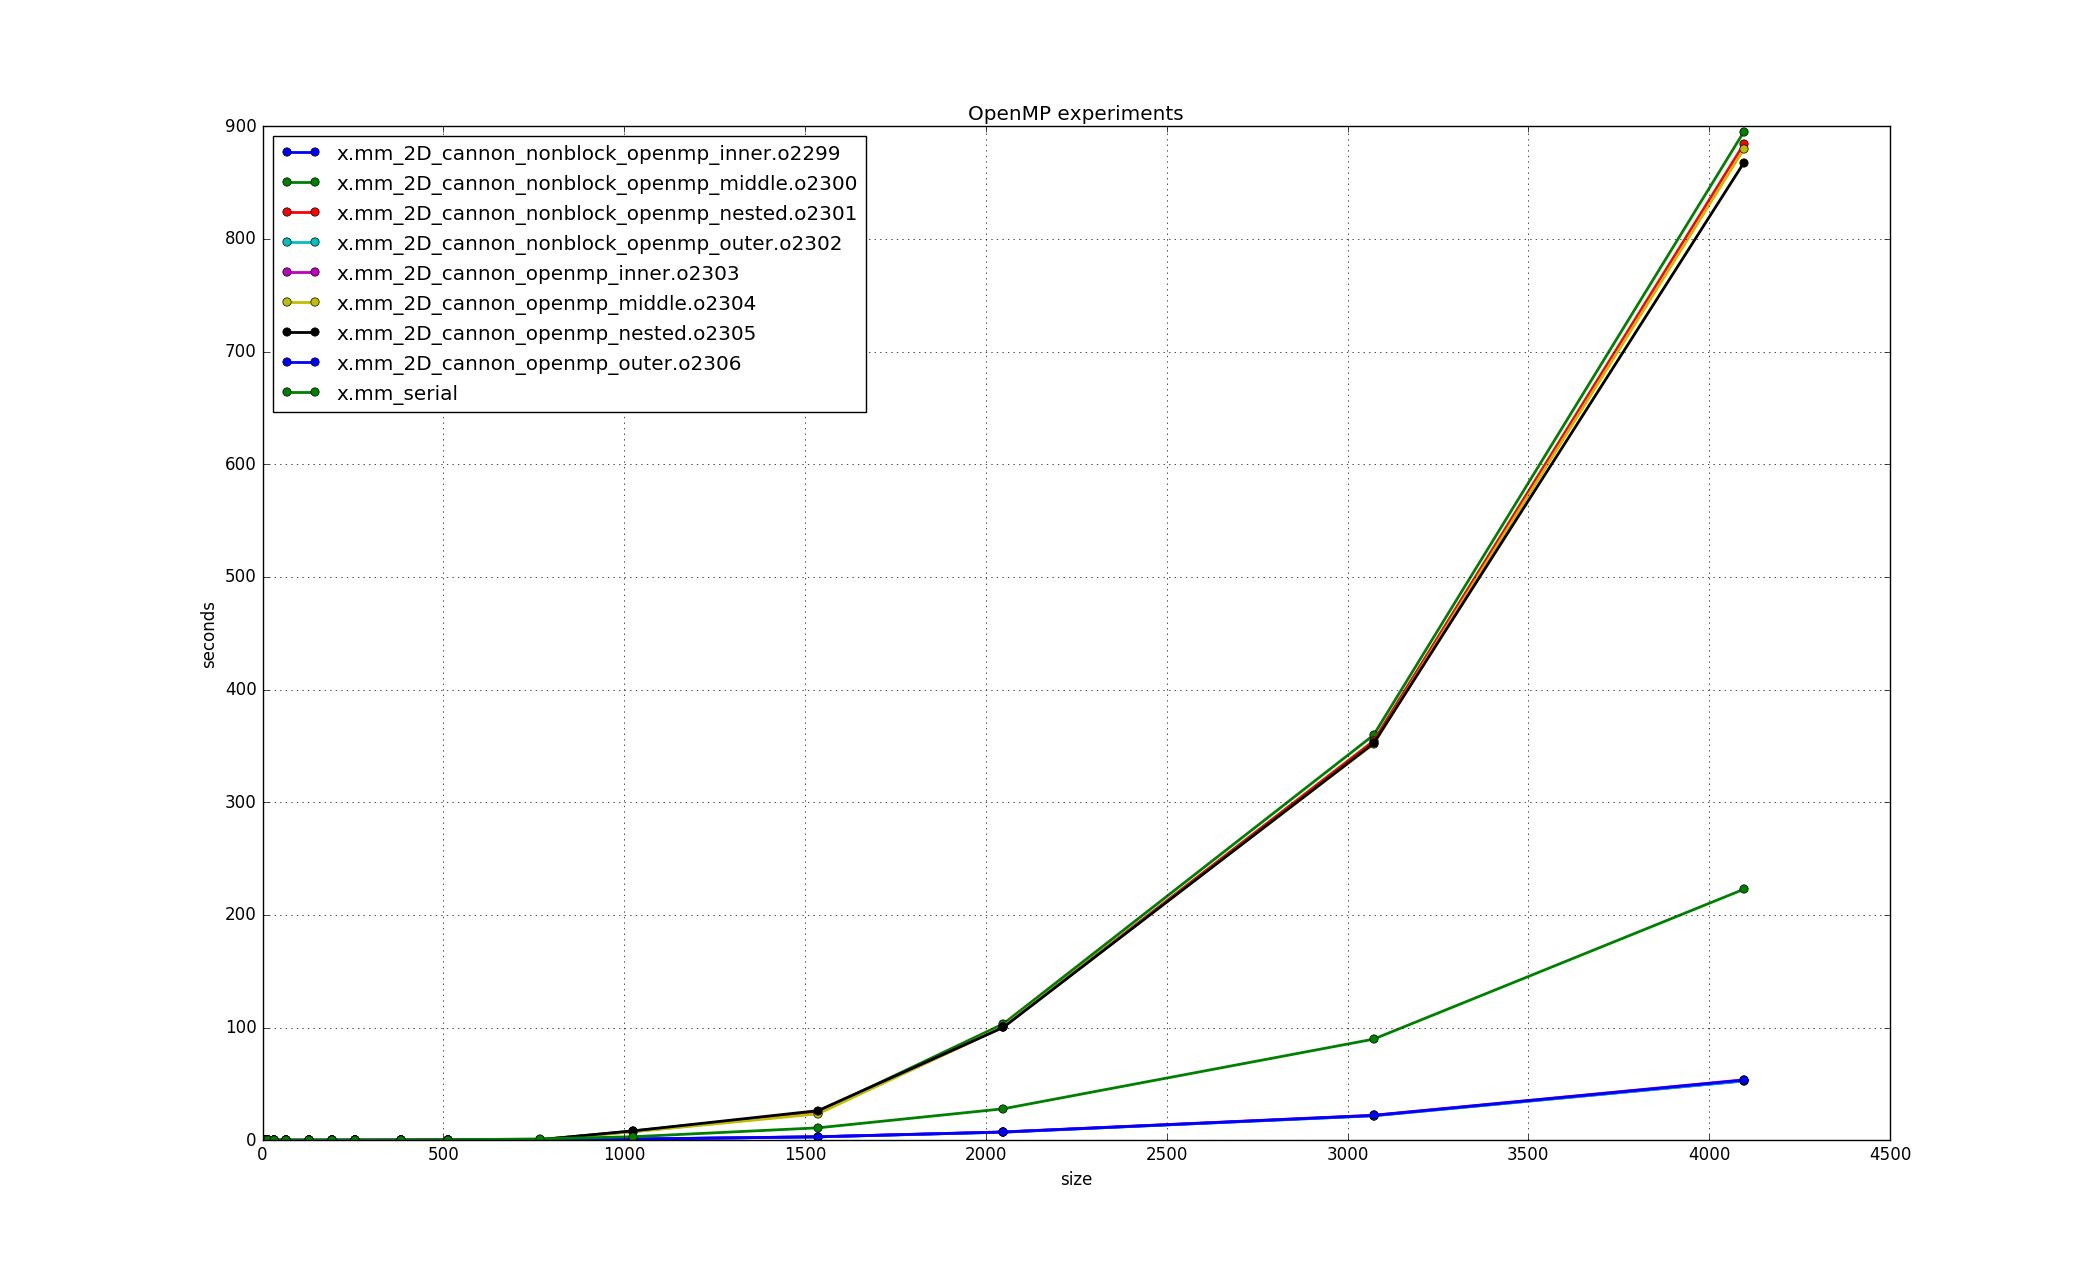
\includegraphics[width=15cm]{immagini/openmp_times.png}
    \end{center}
    \caption{MM MPI with OpenMP: tempo di esecuzione}
    \label{fig:openmp_times}
\end{figure}

\begin{figure}[htbp]
    \begin{center}
        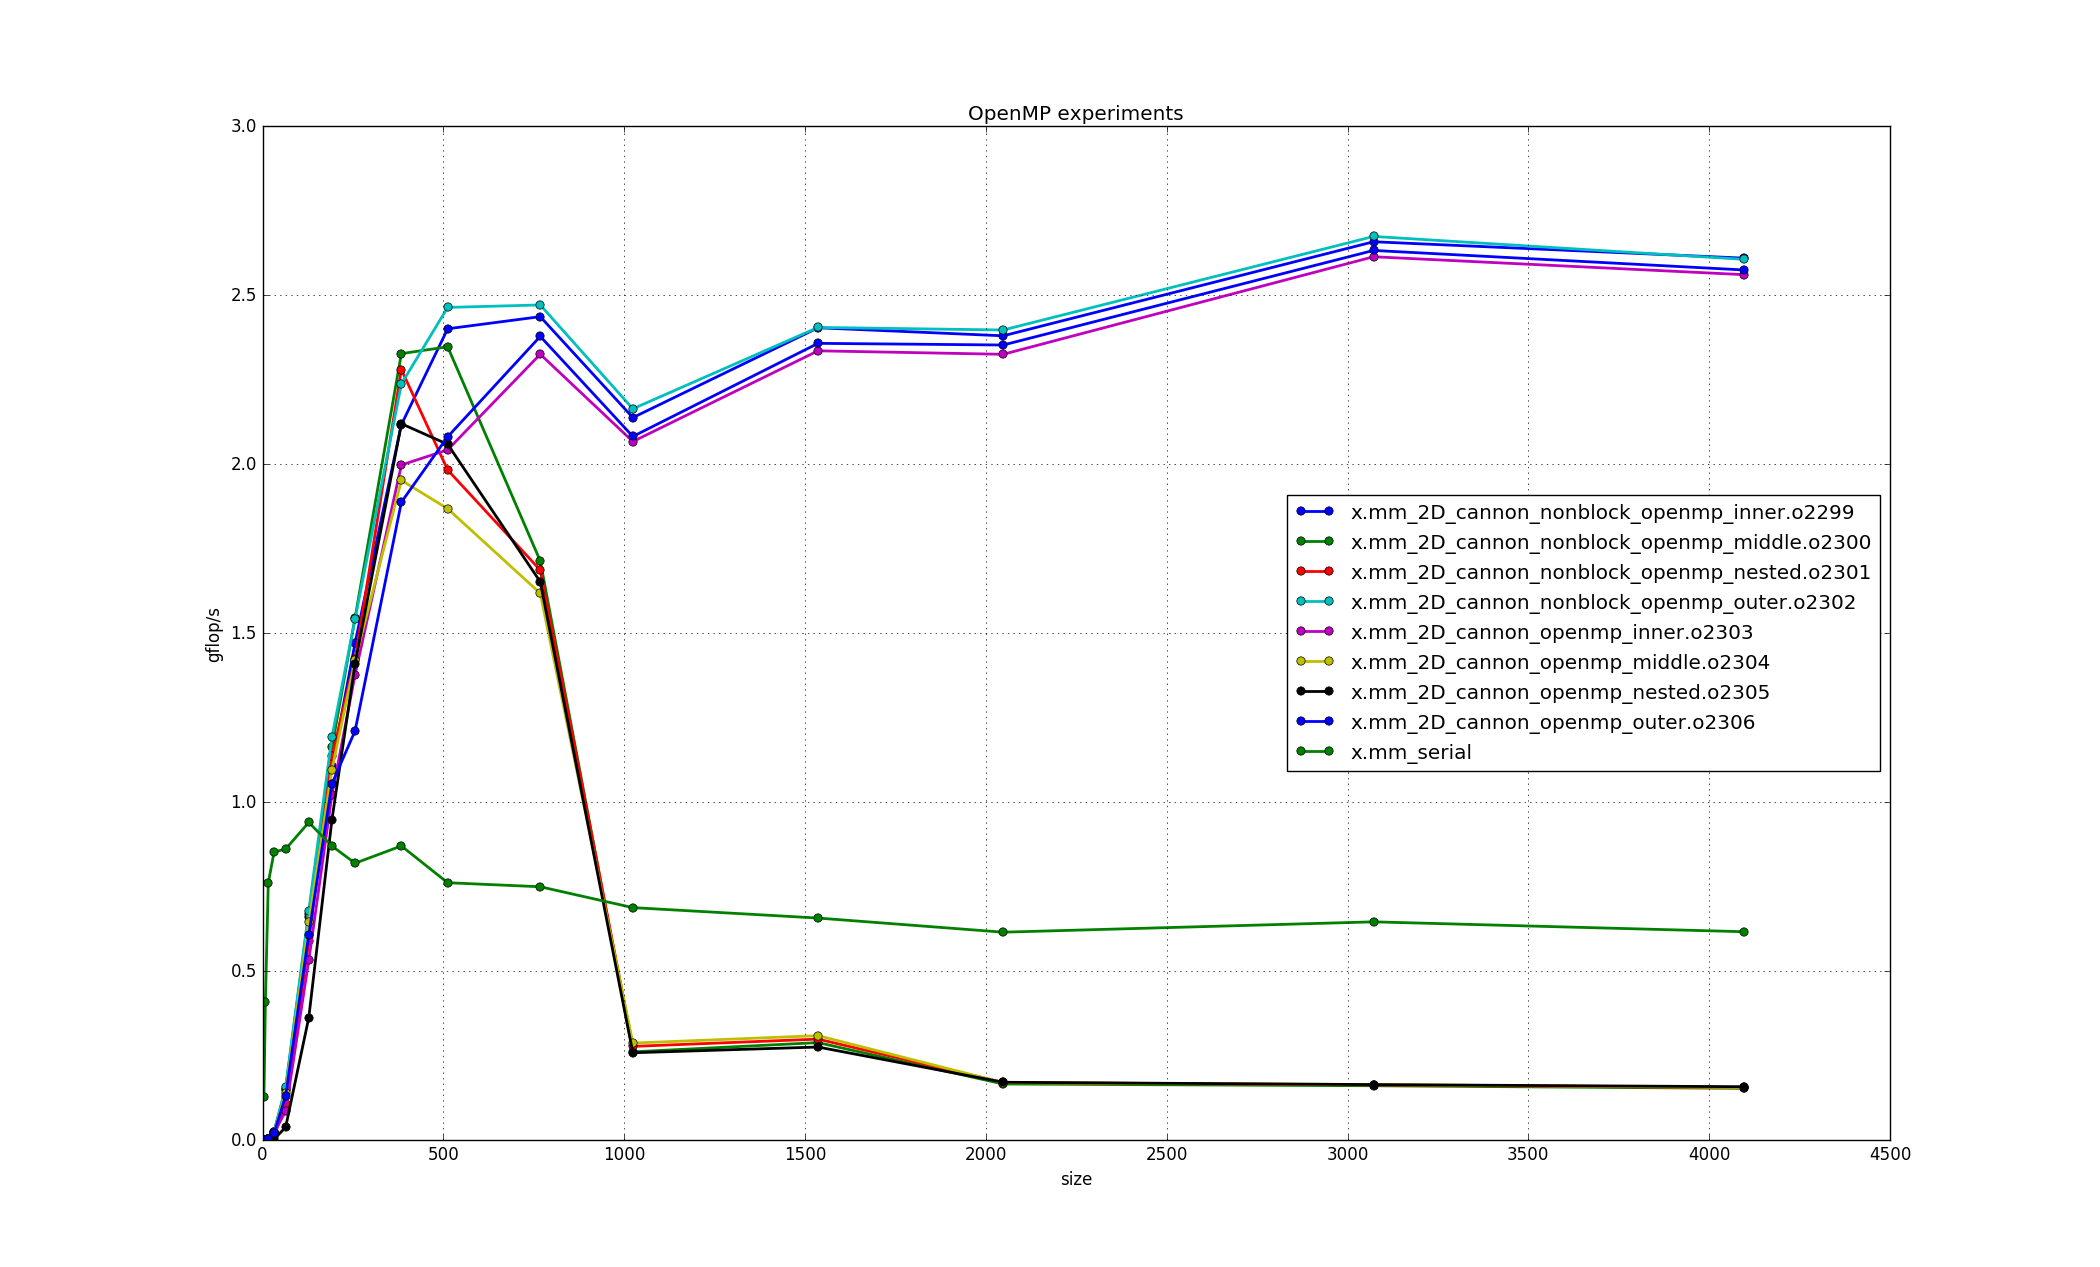
\includegraphics[width=15cm]{immagini/openmp_gflops.png}
    \end{center}
    \caption{MM MPI with OpenMP: Gflop/s}
    \label{fig:openmp_gflops}
\end{figure}

\paragraph{Speedup ed efficienza}

Calcolare speedup ed efficienza per OpenMP

\subsection{MPI con CBLAS}

Le figure \ref{fig:cblas_times} e \ref{fig:cblas_gflops} rappresentano i risultati degli esperimenti con CBLAS.

\begin{figure}[htbp]
    \begin{center}
        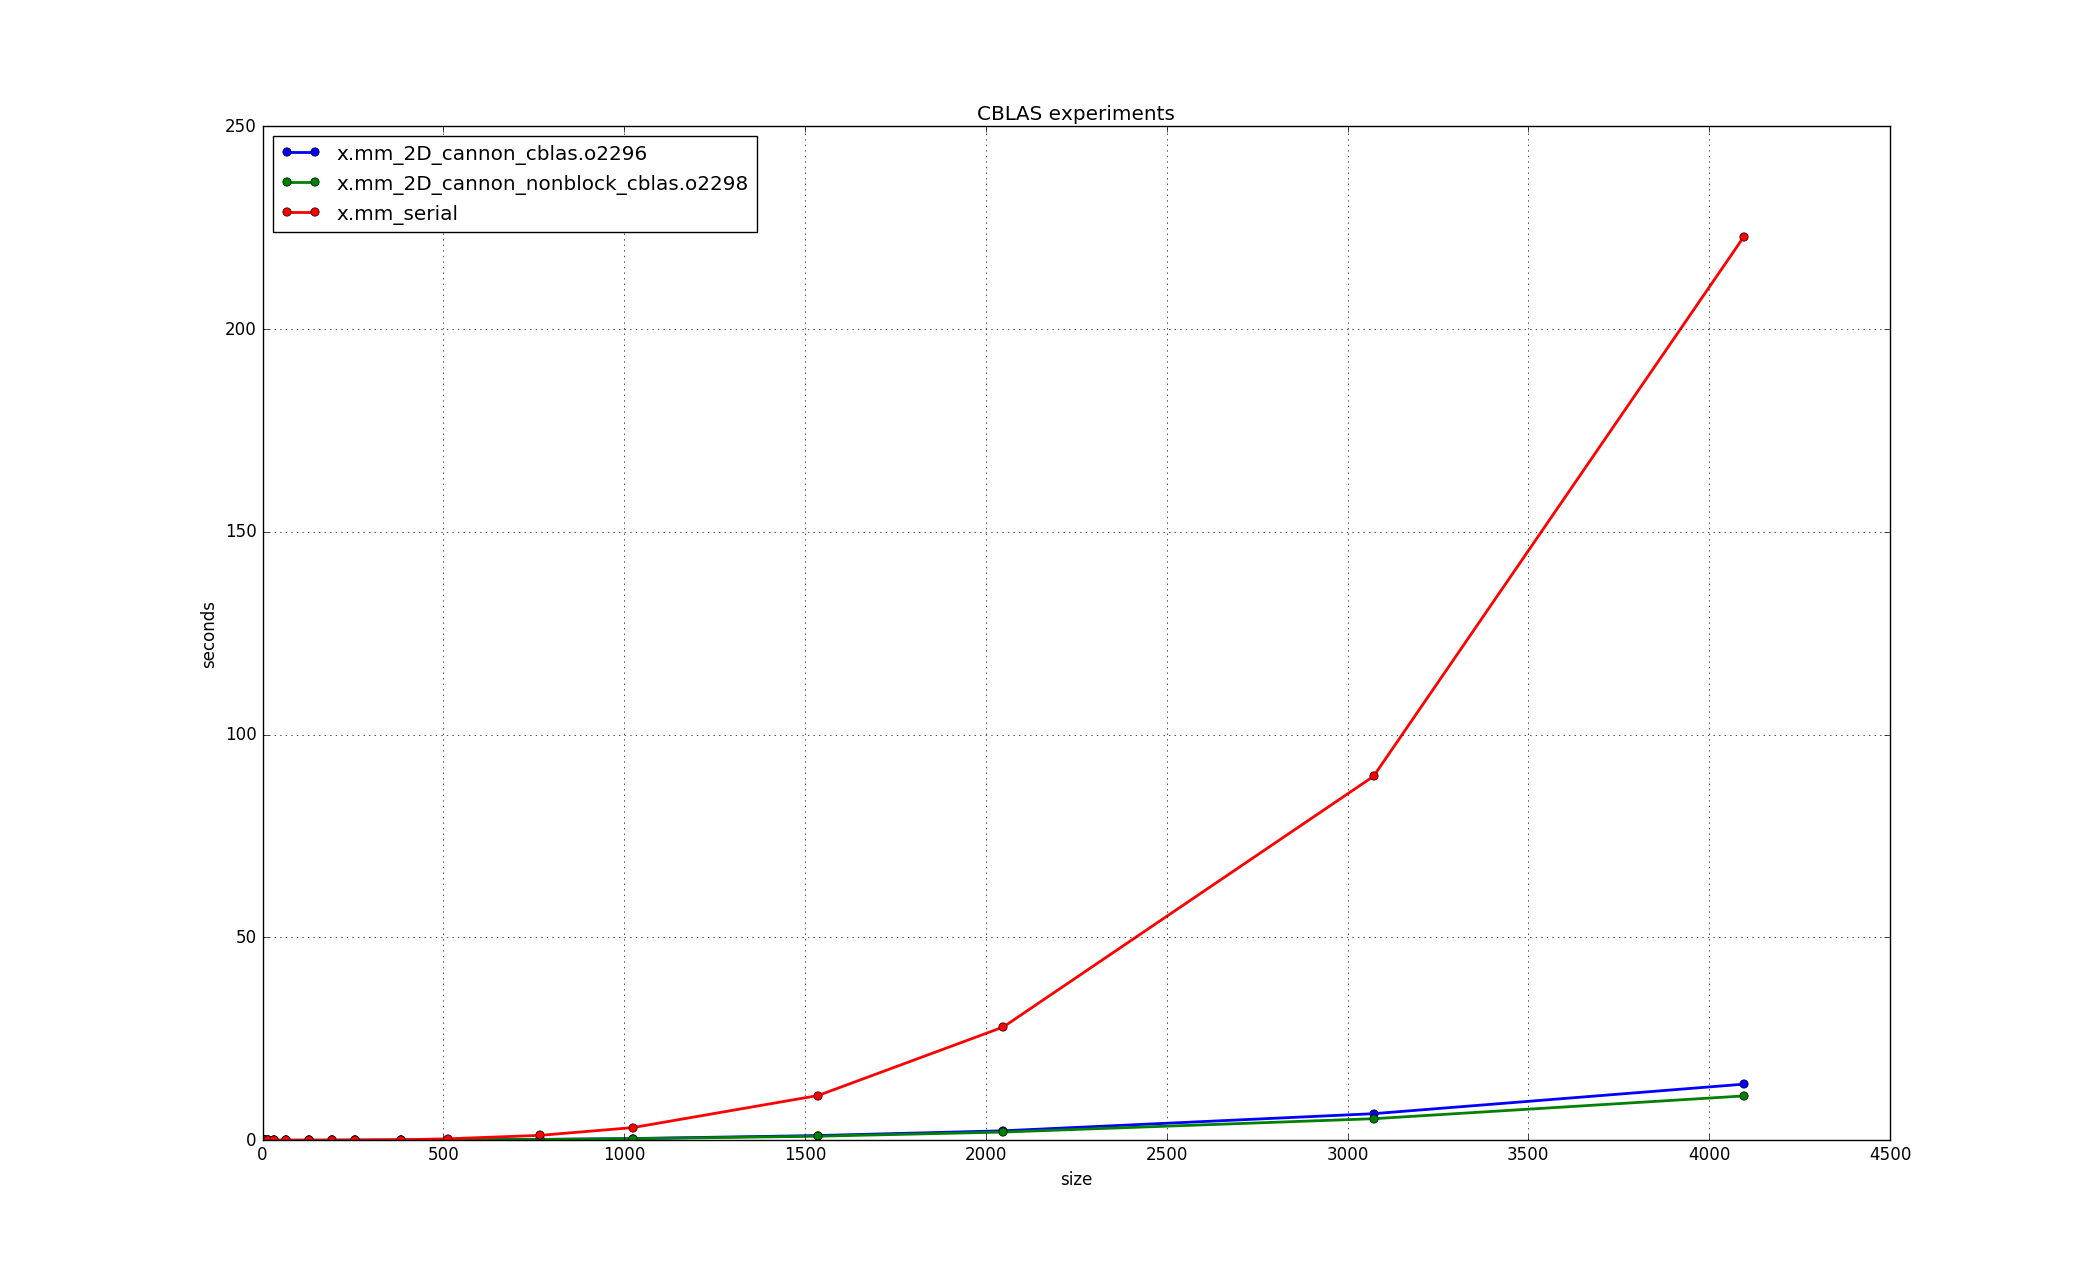
\includegraphics[width=15cm]{immagini/cblas_times.png}
    \end{center}
    \caption{MM MPI with CBLAS: tempo di esecuzione}
    \label{fig:cblas_times}
\end{figure}

\begin{figure}[htbp]
    \begin{center}
        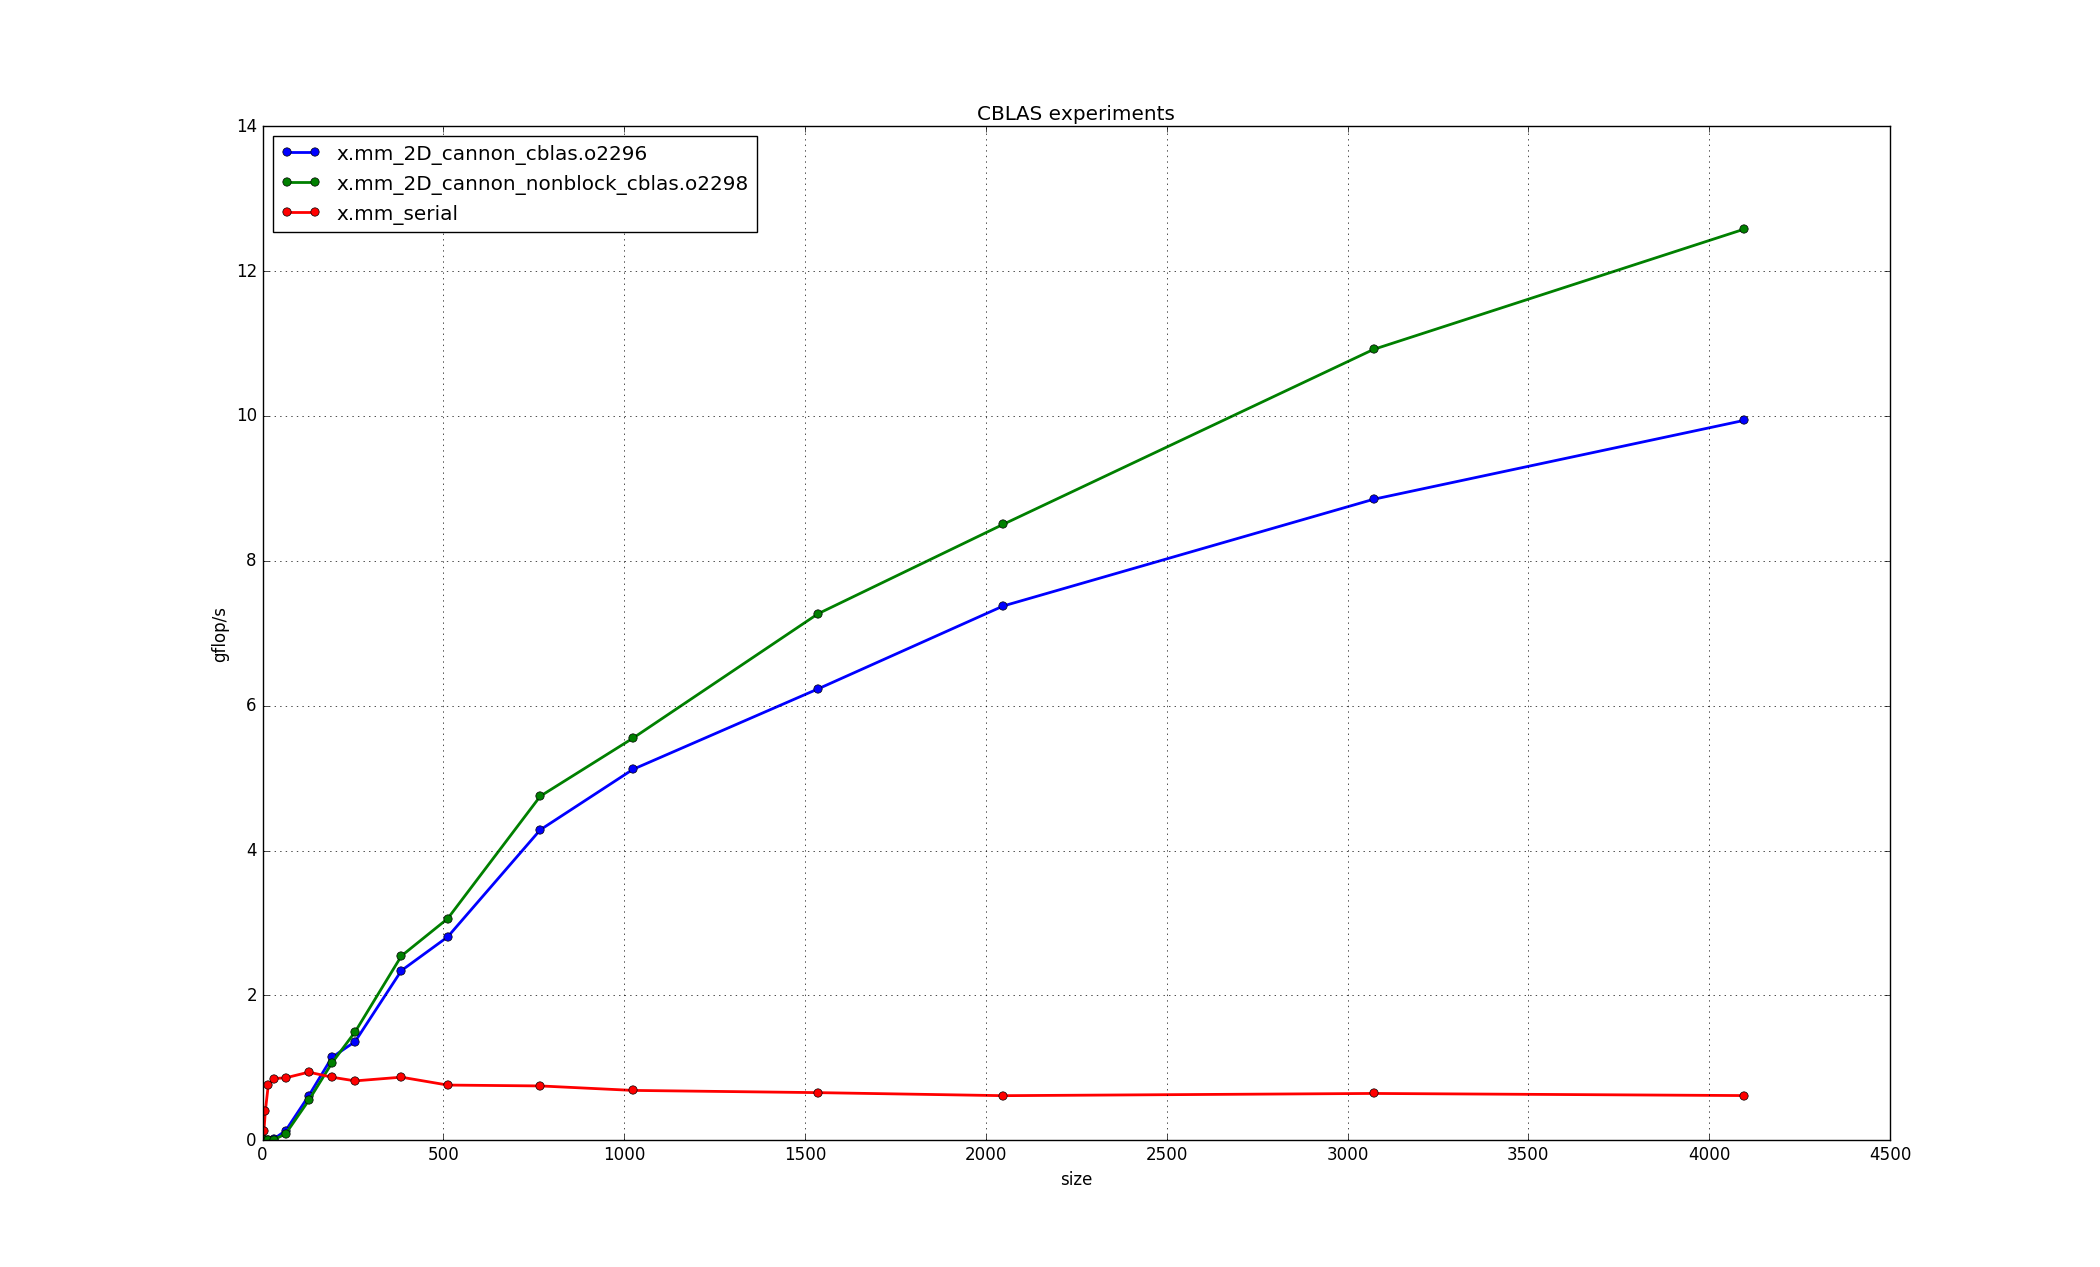
\includegraphics[width=15cm]{immagini/cblas_gflops.png}
    \end{center}
    \caption{MM MPI with CBLAS: Gflop/s}
    \label{fig:cblas_gflops}
\end{figure}

\paragraph{Speedup ed efficienza}
Calcolare speedup ed efficienza per CBLAS

\subsection{Visioni di insieme}
In questa ultima sezione si ha una visione di insieme su tutti esperimenti effettuati (figure \ref{fig:all_times} e \ref{fig:all_gflops}.

\begin{figure}[htbp]
    \begin{center}
        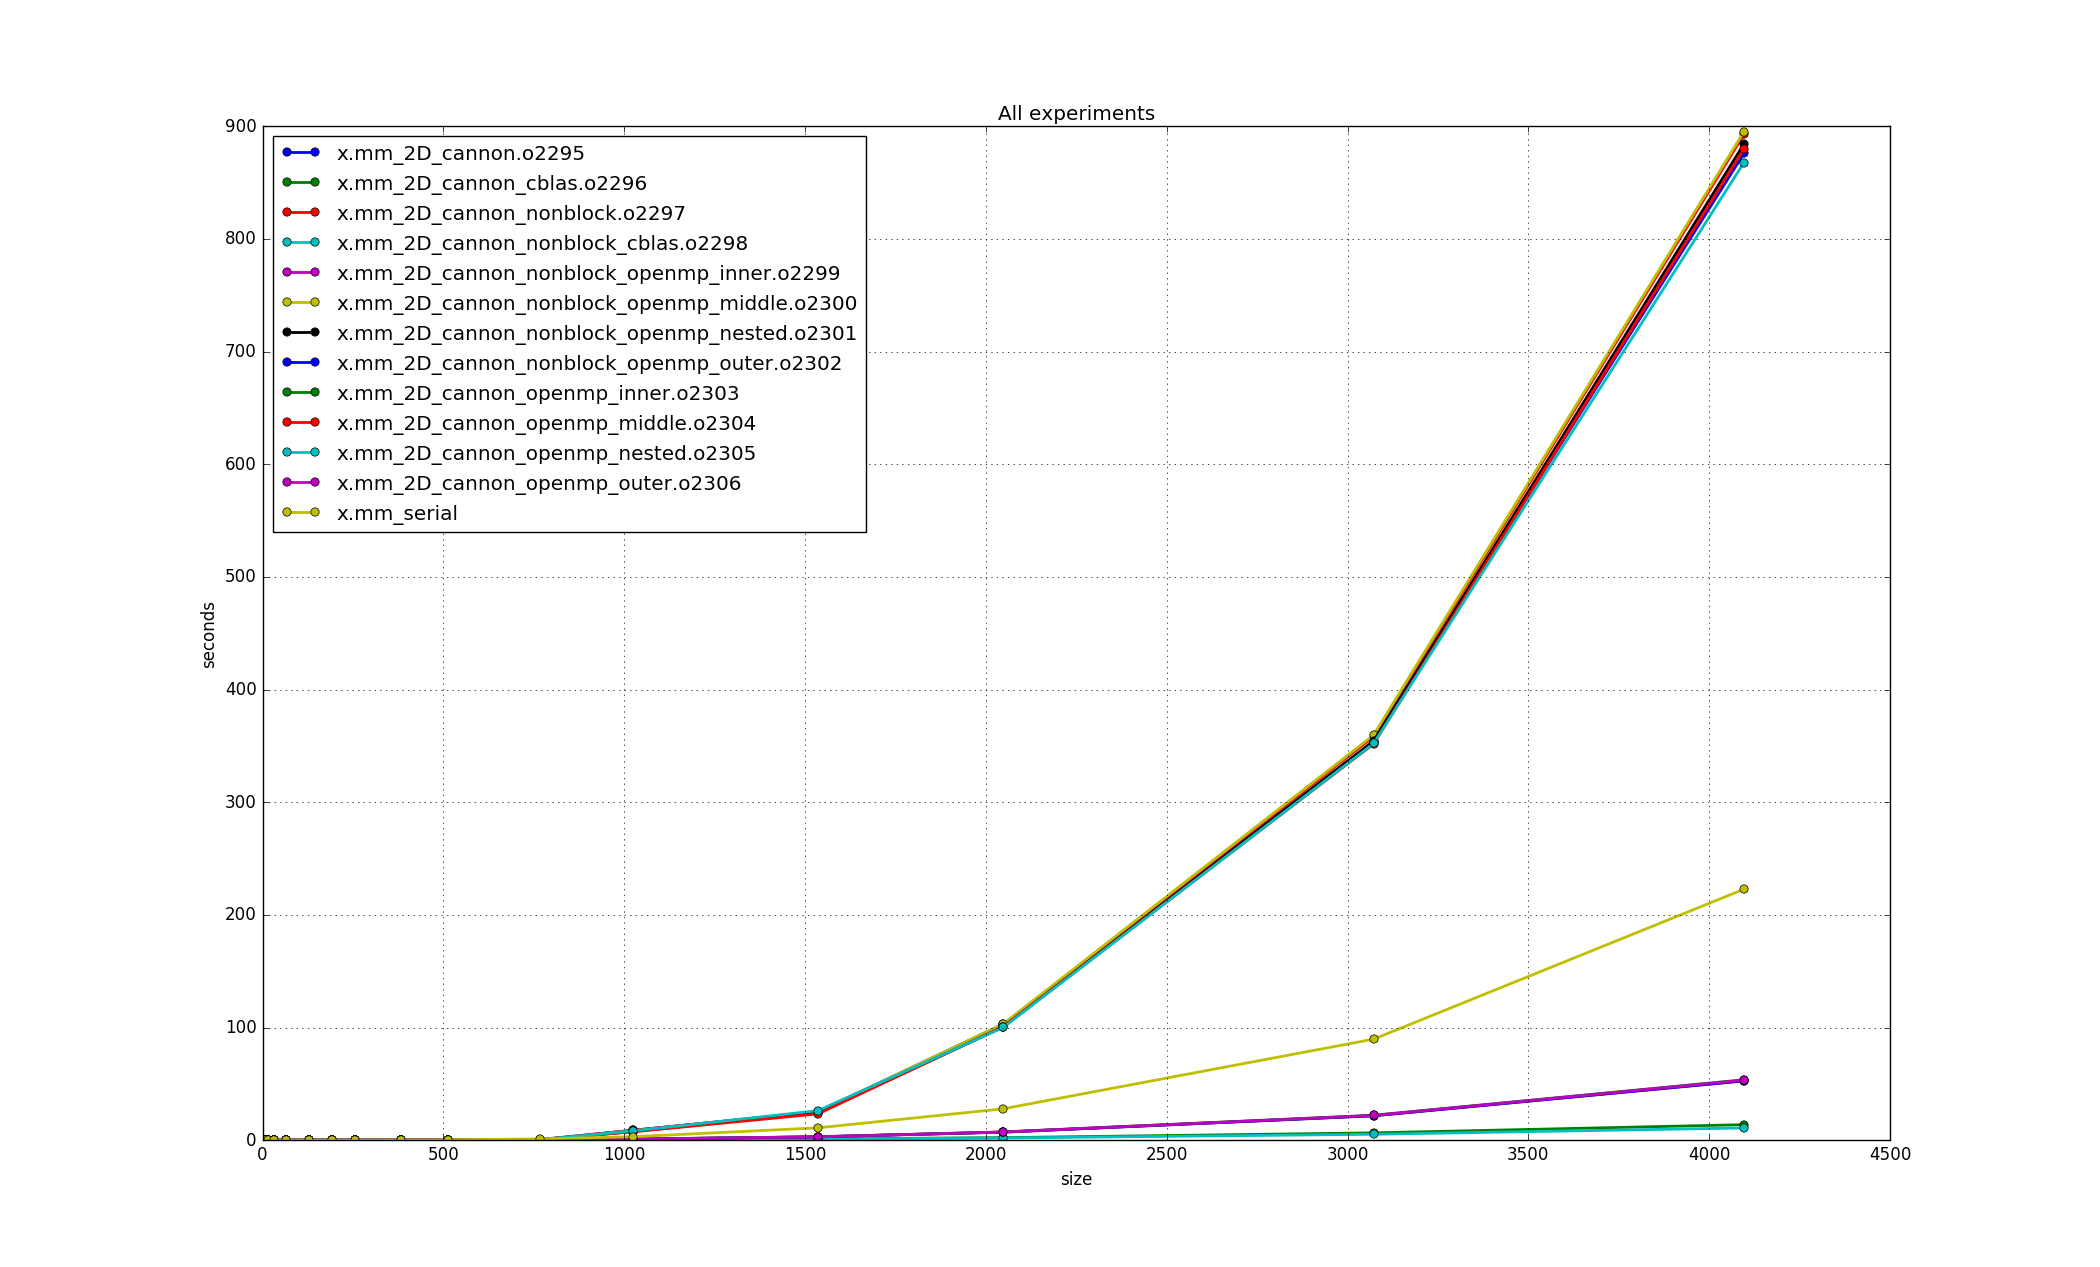
\includegraphics[width=15cm]{immagini/all_times.png}
    \end{center}
    \caption{MM MPI: tempo di esecuzione}
    \label{fig:all_times}
\end{figure}

\begin{figure}[htbp]
    \begin{center}
        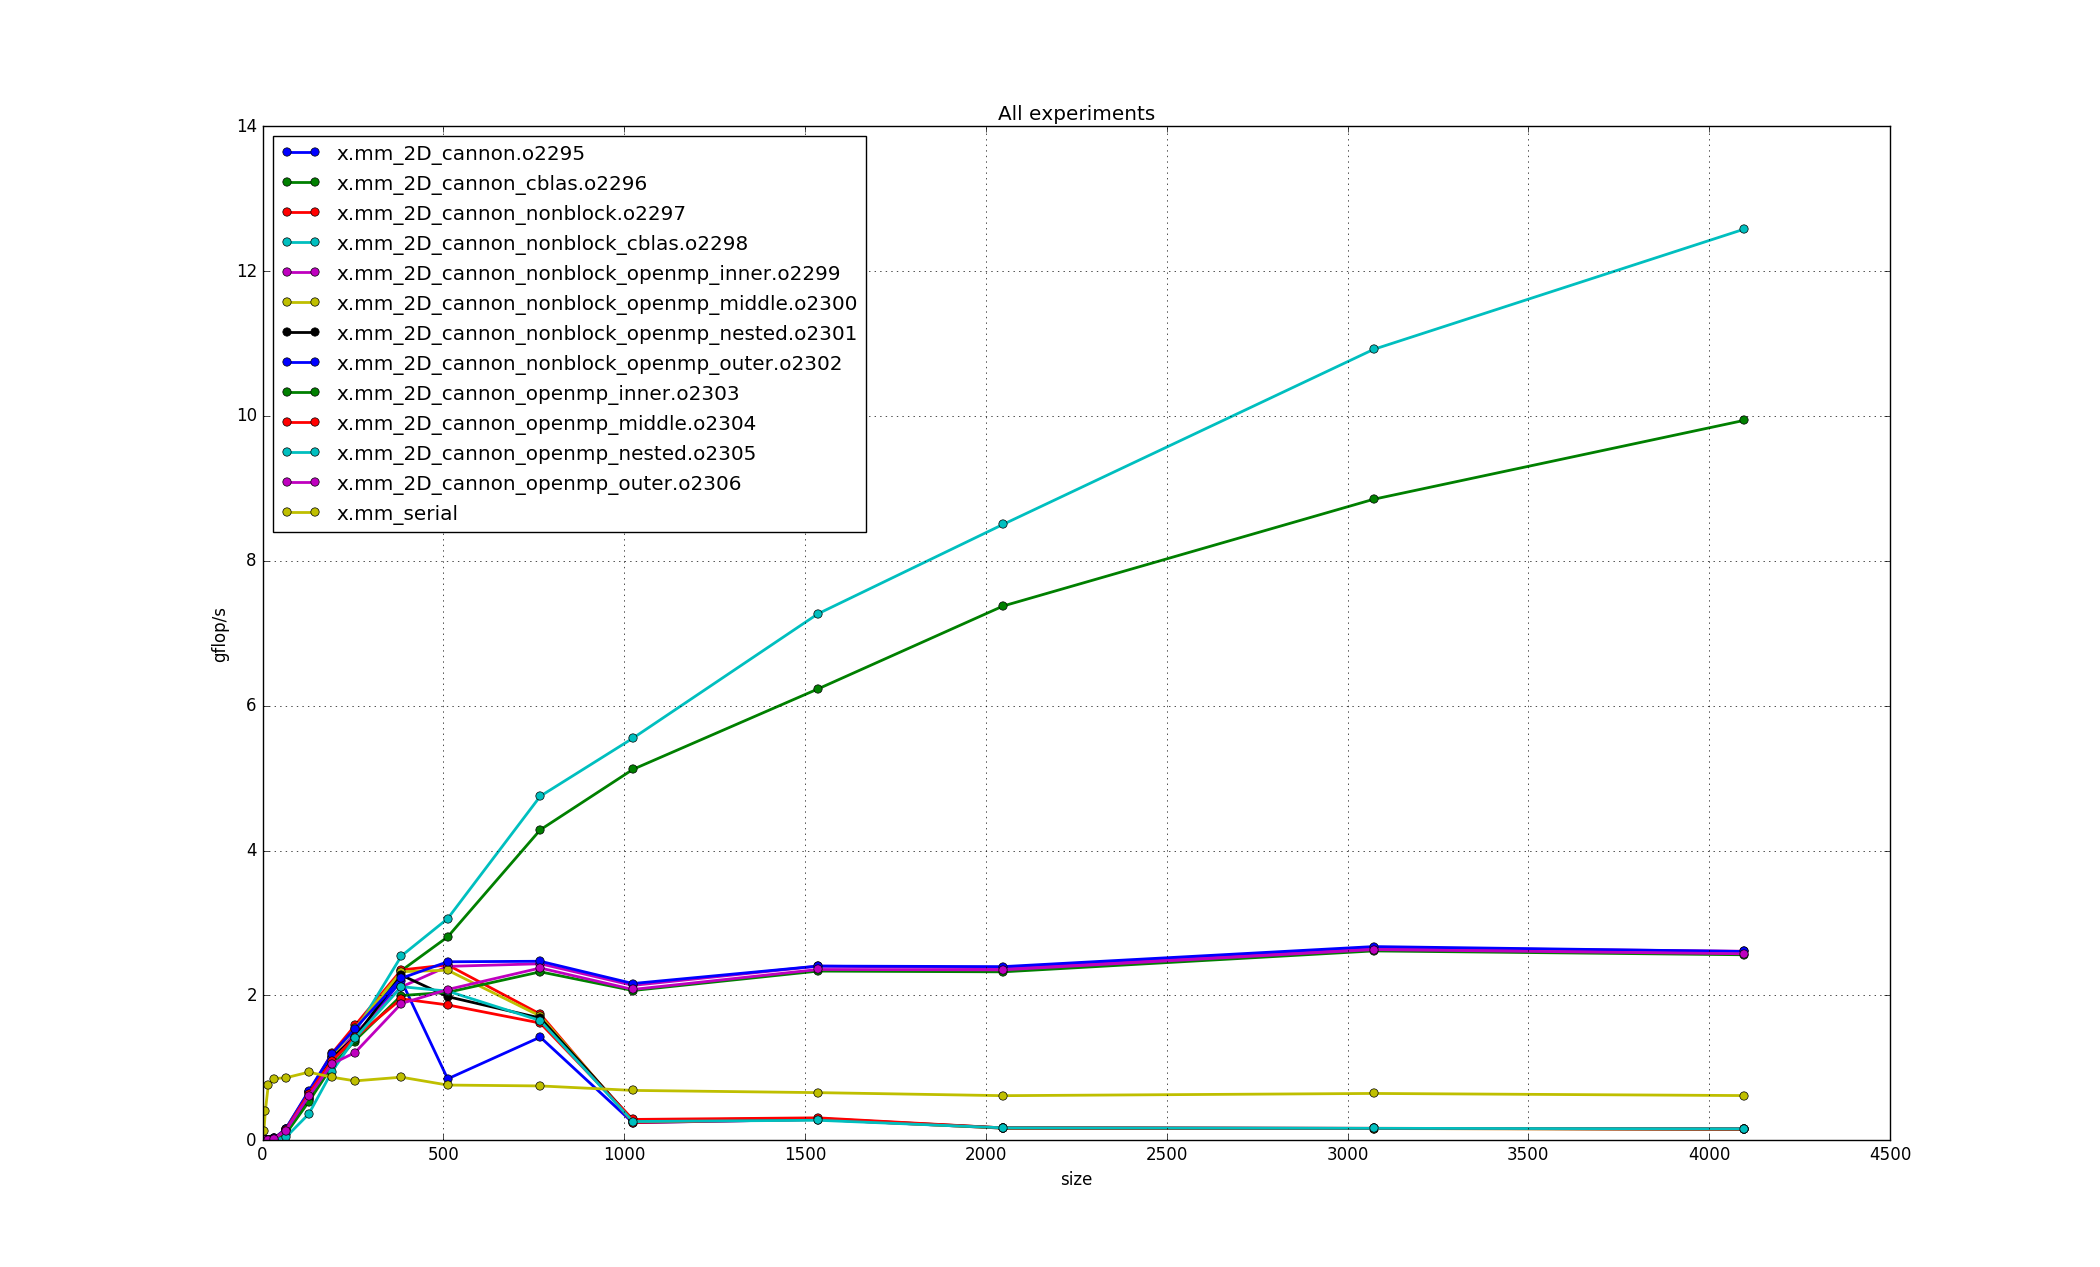
\includegraphics[width=15cm]{immagini/all_gflops.png}
    \end{center}
    \caption{MM MPI: Gflop/s}
    \label{fig:all_gflops}
\end{figure}

\subsection{MPI bloccanti}

Tutti gli esperimenti bloccanti

\begin{figure}[htbp]
    \begin{center}
        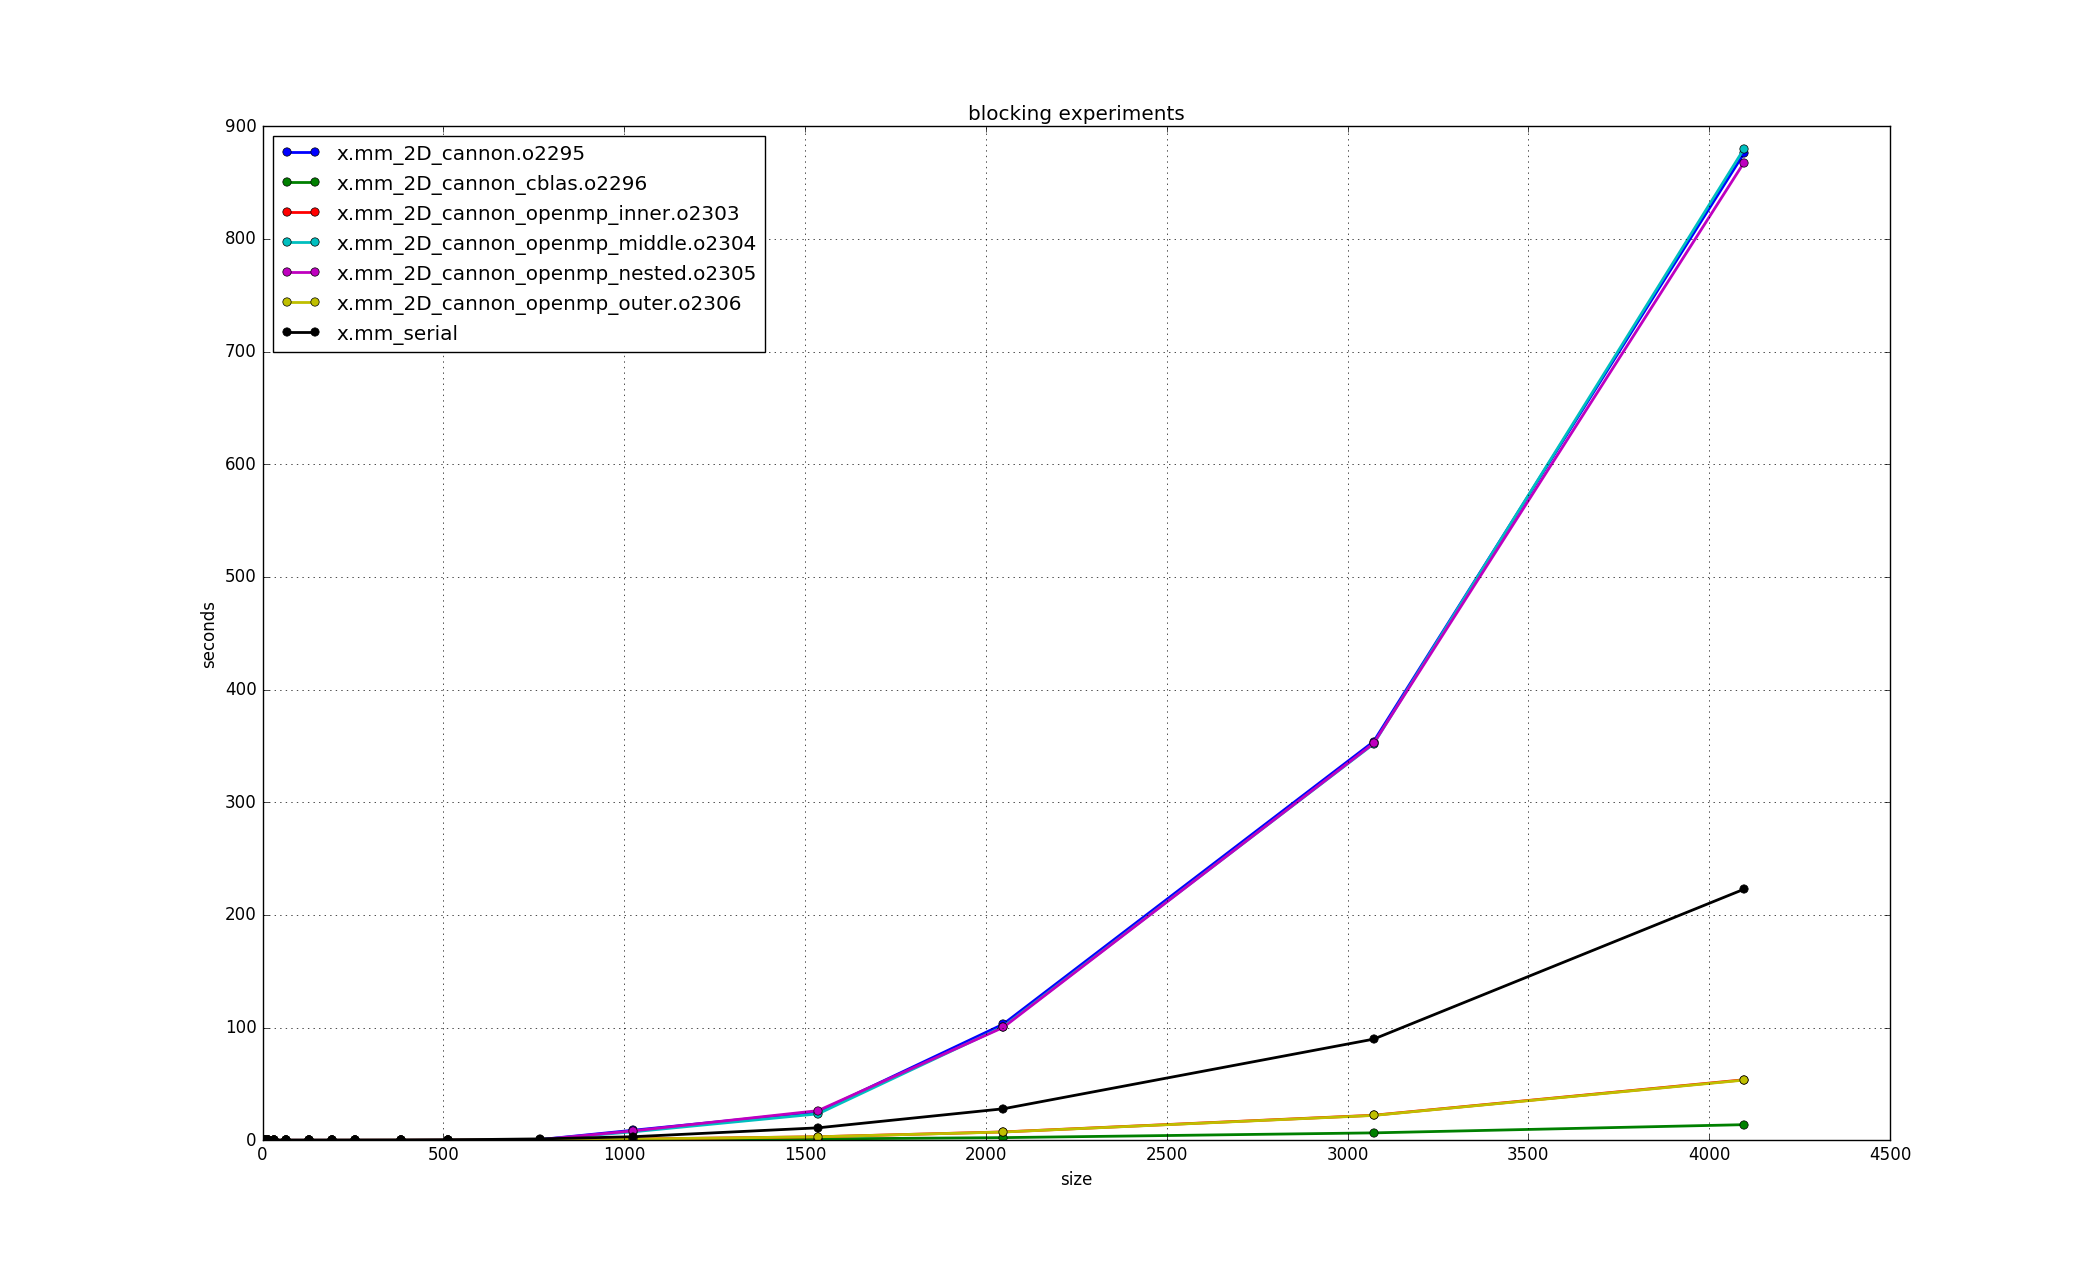
\includegraphics[width=15cm]{immagini/blocking_times.png}
    \end{center}
    \caption{MM MPI bloccanti: tempo di esecuzione}
    \label{fig:blocking_times}
\end{figure}

\begin{figure}[htbp]
    \begin{center}
        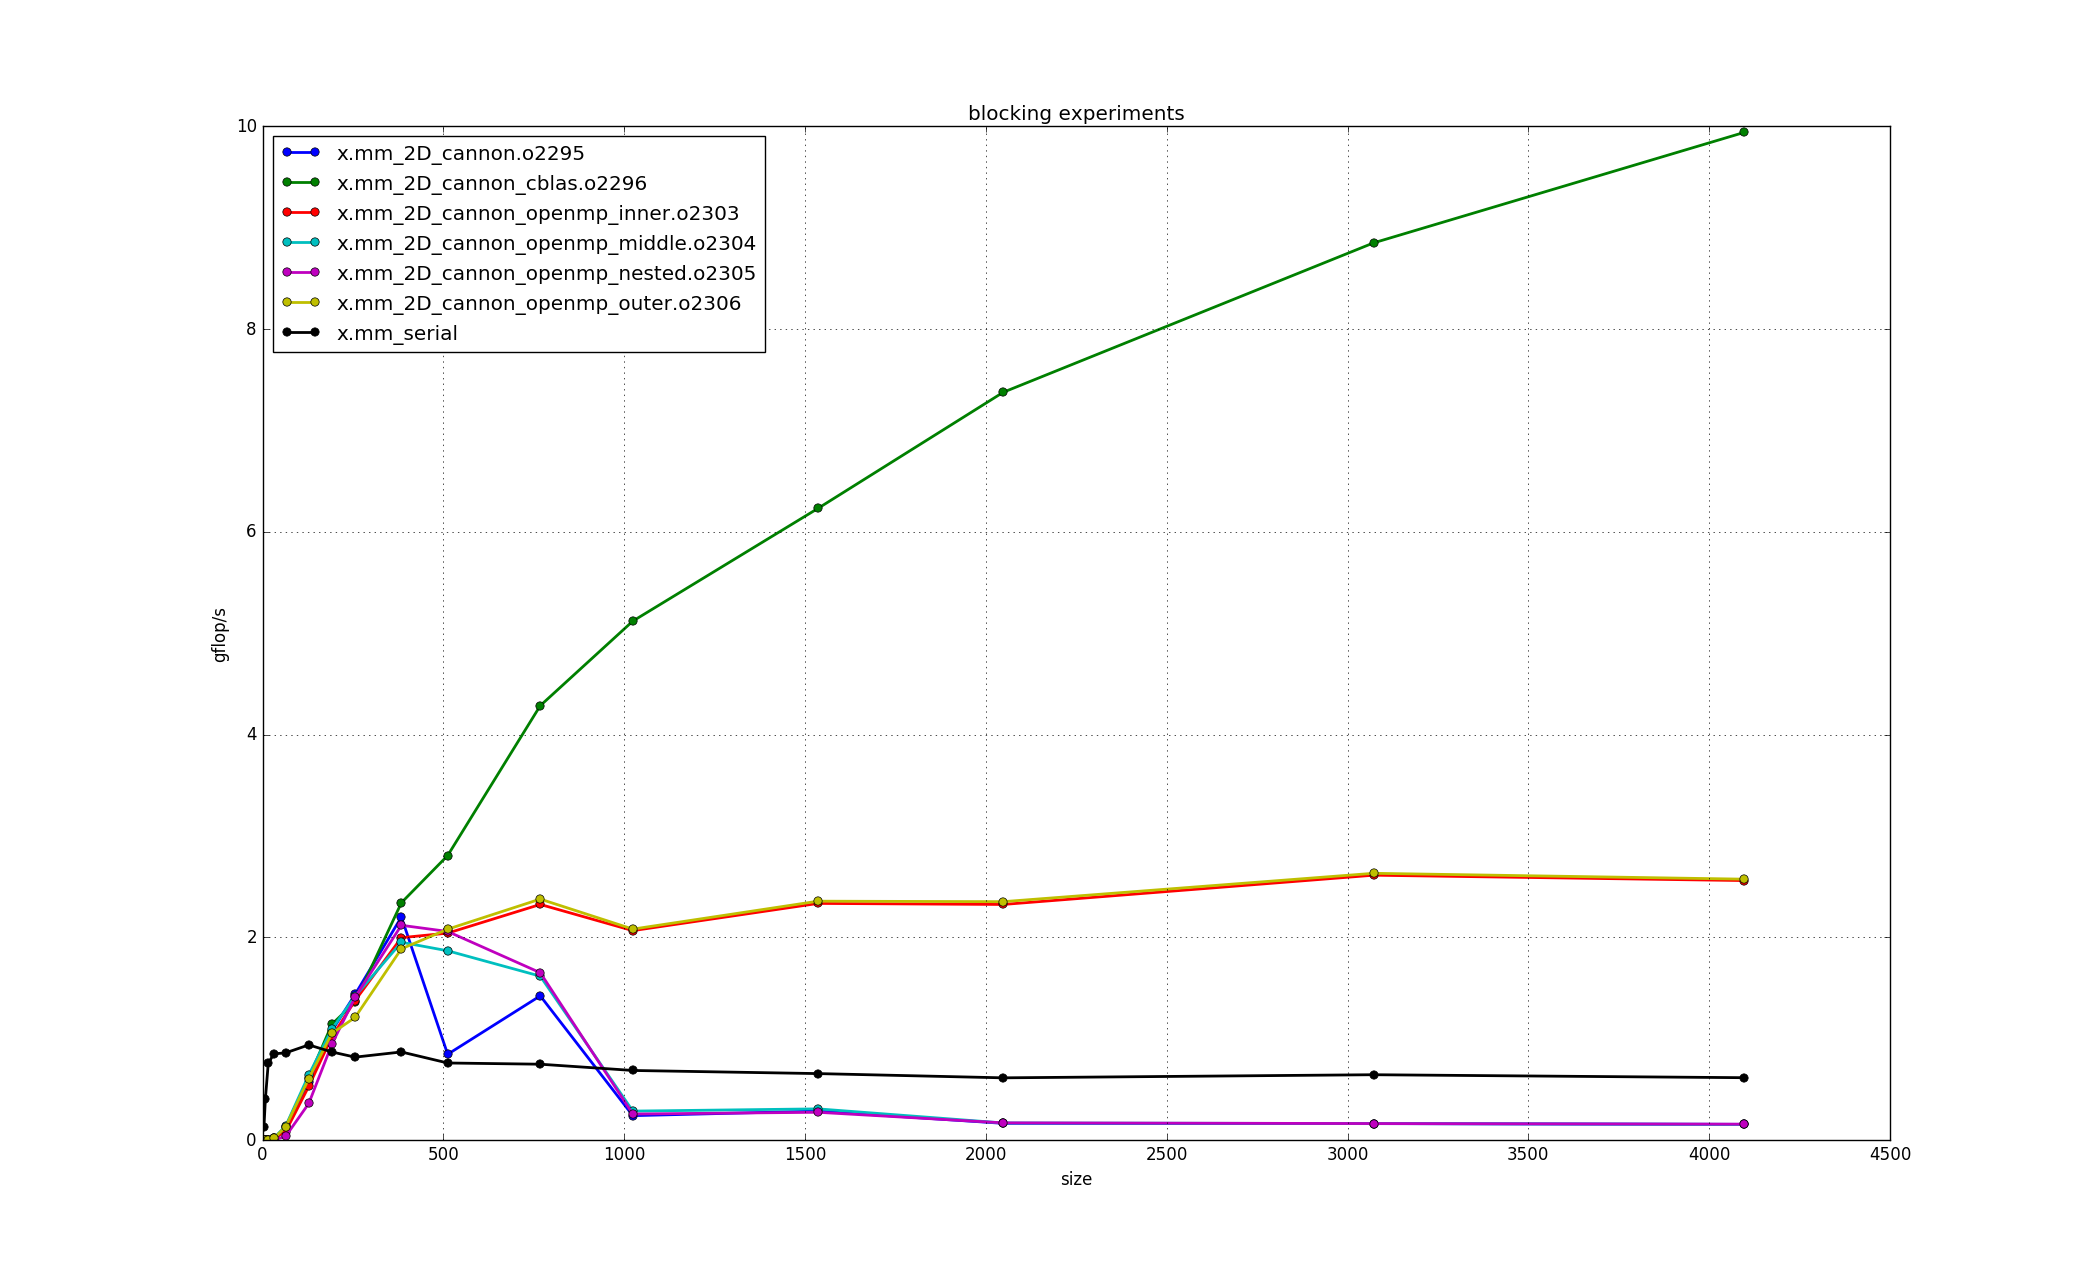
\includegraphics[width=15cm]{immagini/blocking_gflops.png}
    \end{center}
    \caption{MM MPI bloccanti: Gflop/s}
    \label{fig:blocking_gflops}
\end{figure}

\subsection{MPI NON bloccanti}

Tutti gli esperimenti NON bloccanti

\begin{figure}[htbp]
    \begin{center}
        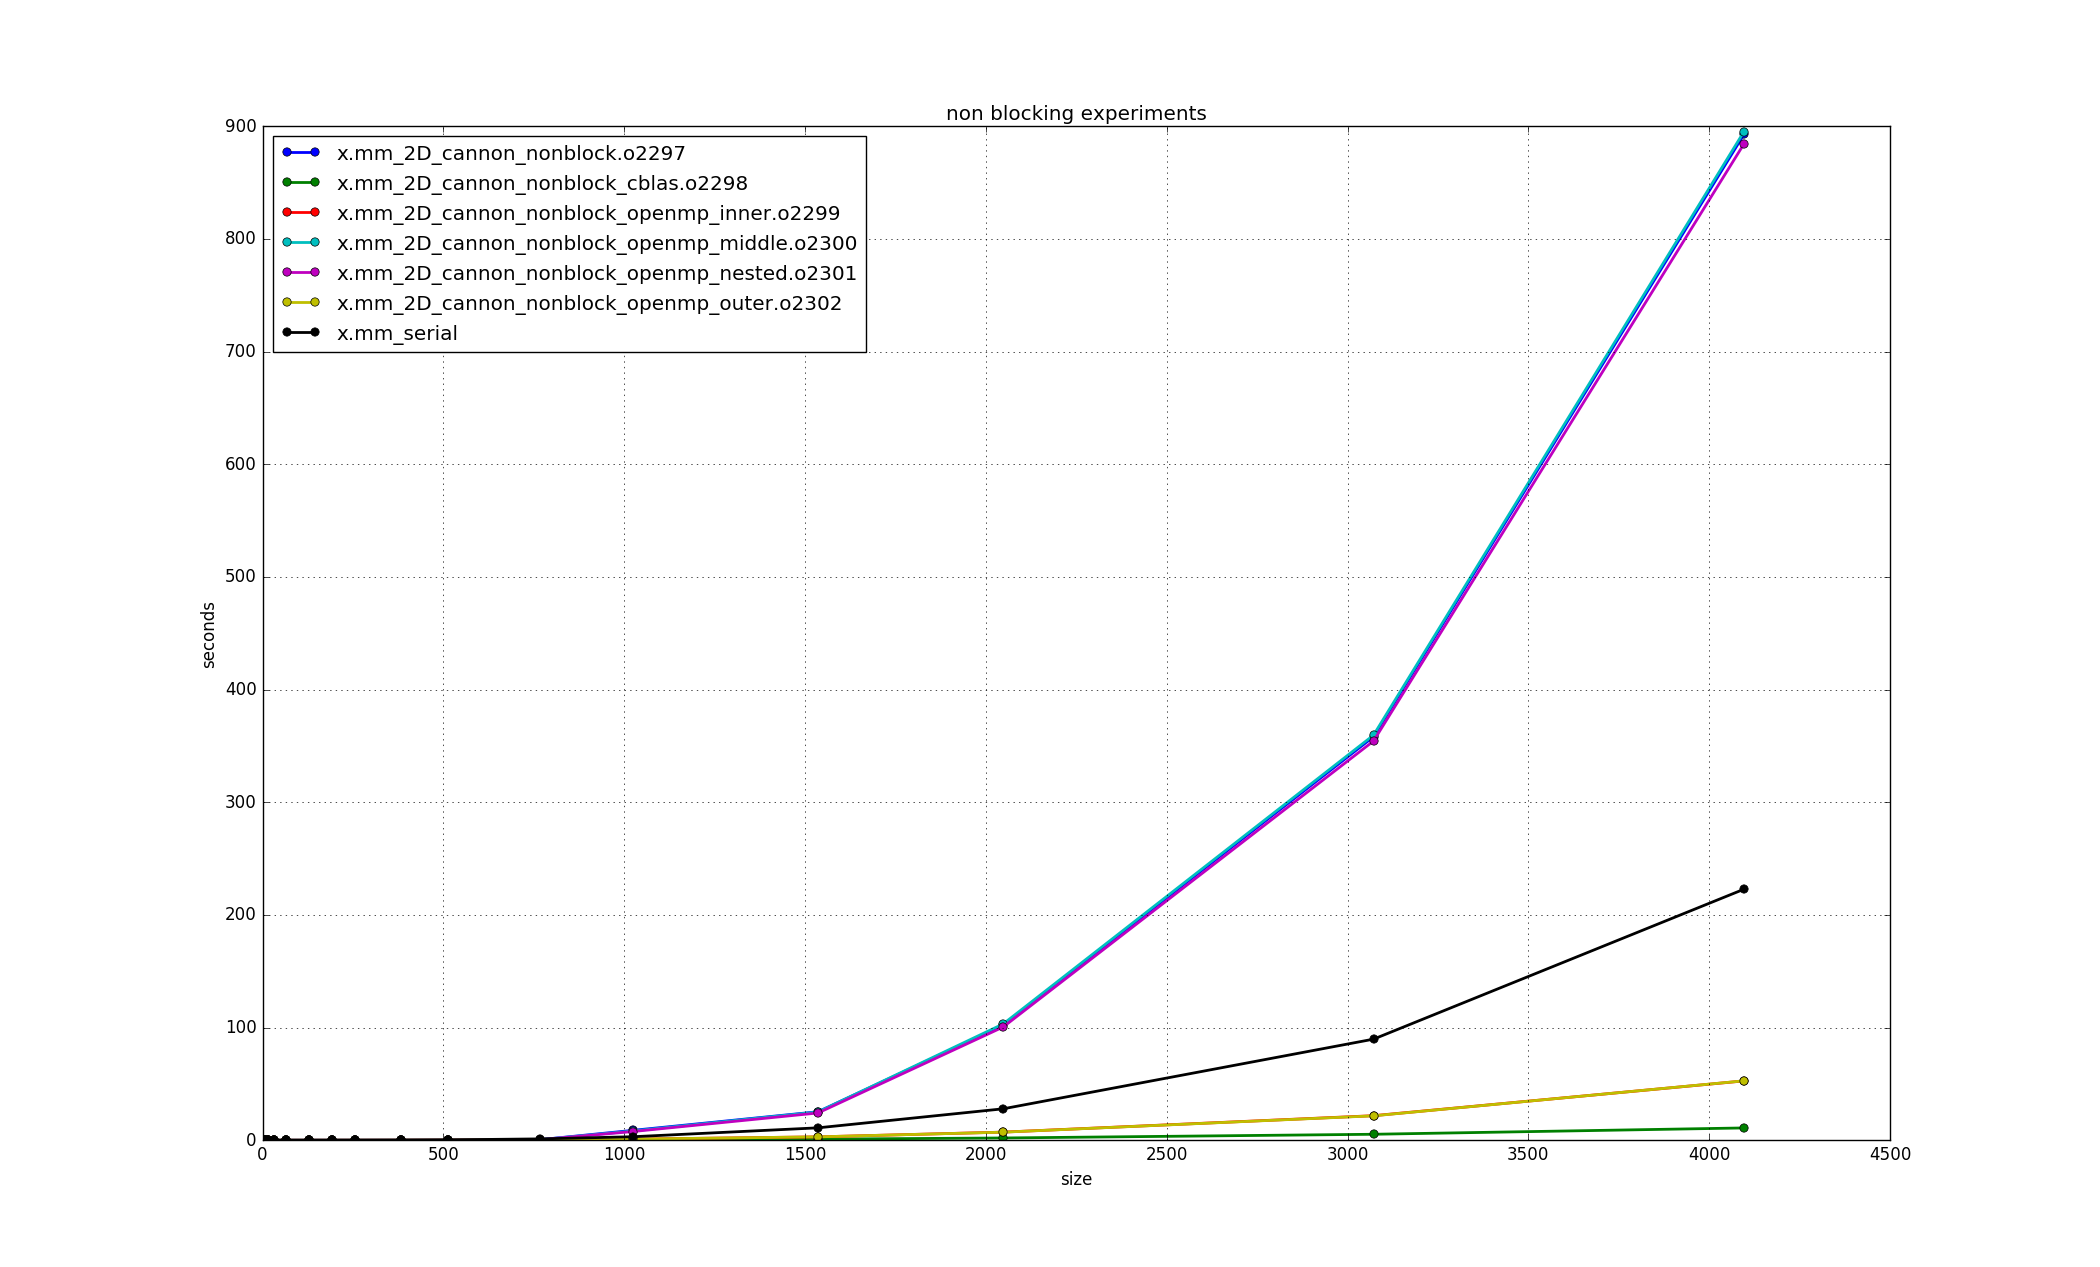
\includegraphics[width=15cm]{immagini/non_blocking_times.png}
    \end{center}
    \caption{MM MPI NON bloccanti: tempo di esecuzione}
    \label{fig:non_blocking_times}
\end{figure}

\begin{figure}[htbp]
    \begin{center}
        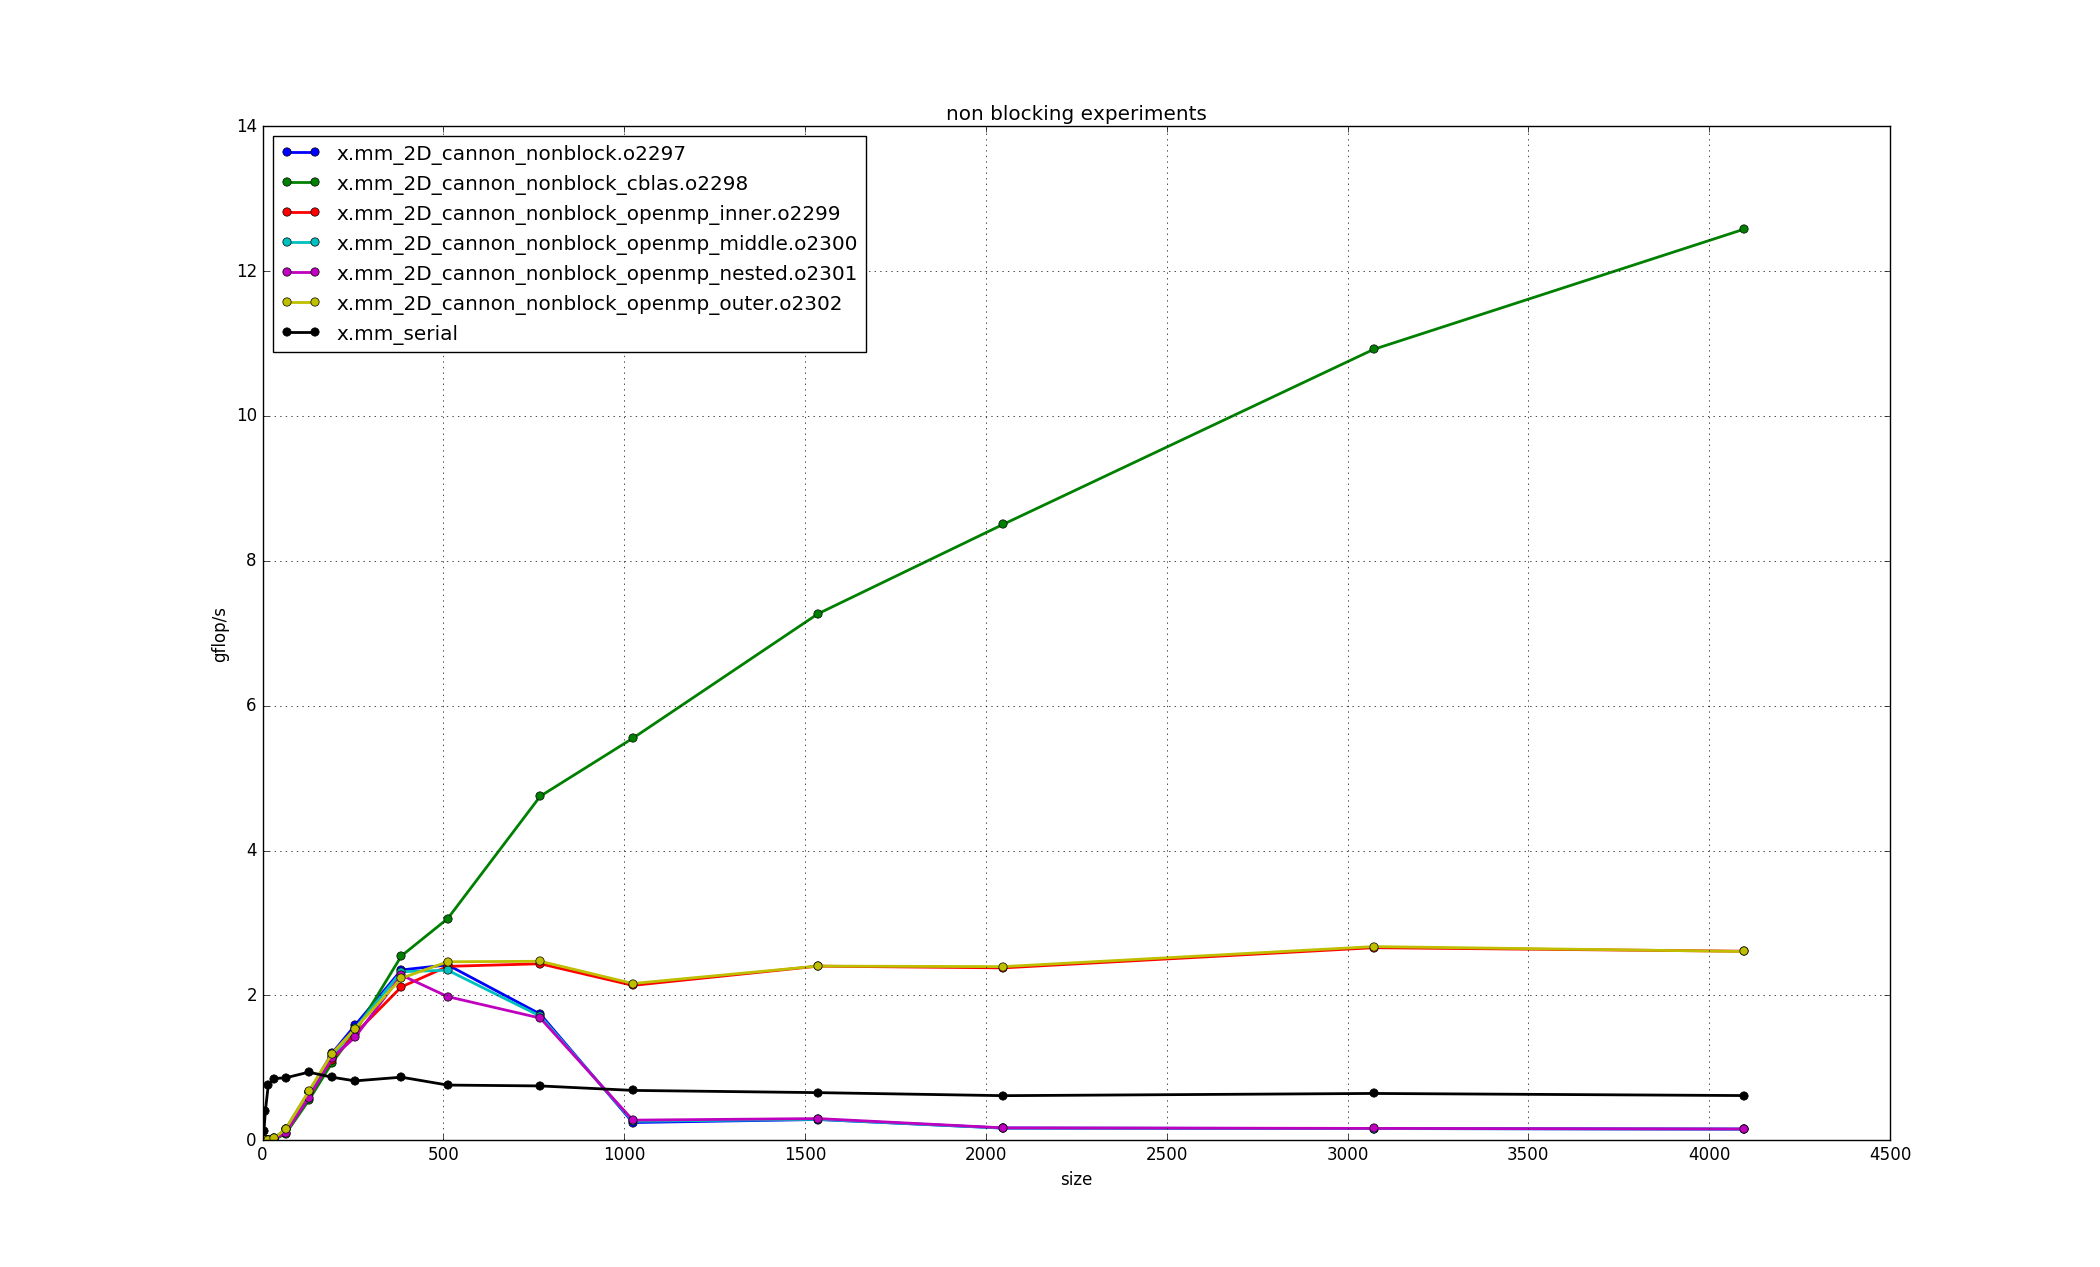
\includegraphics[width=15cm]{immagini/non_blocking_gflops.png}
    \end{center}
    \caption{MM MPI bloccanti: Gflop/s}
    \label{fig:non_blocking_gflops}
\end{figure}
